\section{Modelling with UML}
\subsection{Primary Software architecture}
\subsubsection{Component segmentation and description of interfaces}
The purpose of the following diagram is to show the structural relationship between the components of the memory stack, to provide a high-level architectural view and to give a rough information about the components.\\
\begin{center}
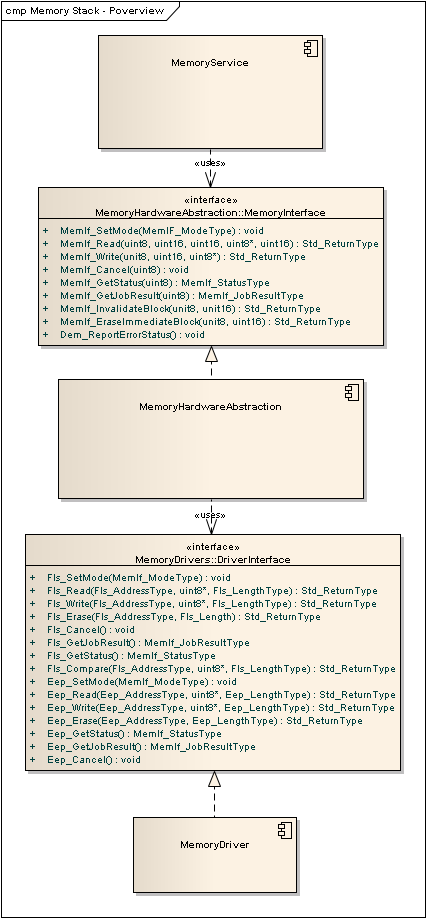
\includegraphics[scale=0.55]{Images/Memory_Stack_POverview.png}
\end{center}
The NVRAM component contains of two main components. They shall provides specific services according to their individual requirements. In particular there is a data management and a maintenance component. The maintenance component is responsible for all loading,writting and saving processes. The data management component is responsible for maintaining  of the non-volite data.
\begin{center}
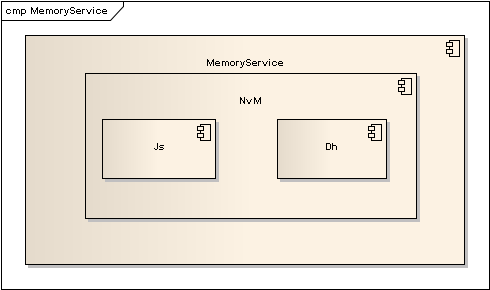
\includegraphics[scale=0.7]{Images/MemoryService_Overview_UML.png}
\end{center}
%\newline
The Abstract memory Interface component allow the NVRAM manager to 
\newline
MemoryAbstractionHardware
\begin{center}
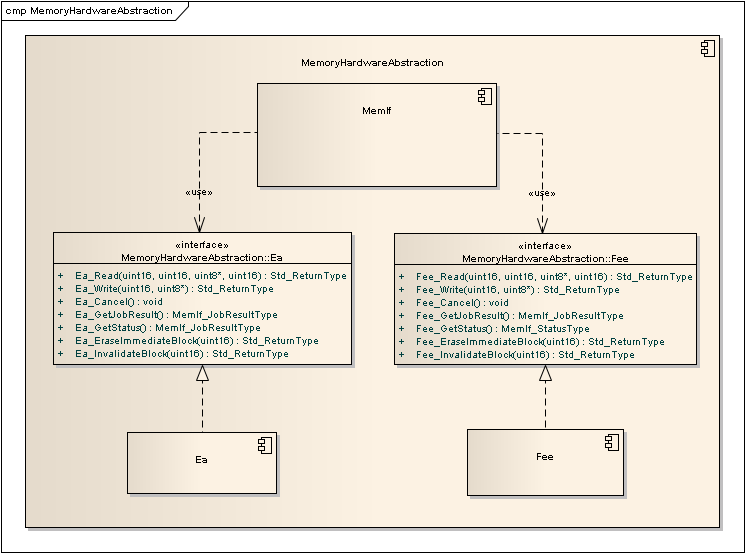
\includegraphics[scale=0.55]{Images/MemoryHardwareAbstraction_Overview_UML.png}
\end{center}


Drivers
\begin{center}
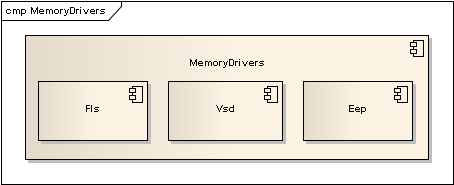
\includegraphics[scale=0.7]{Images/MemoryDrivers_Overview_UML.png}
\end{center}
\subsubsection{Hardware/Software mapping}
\subsubsection{Management of persistent data}
\subsubsection{Access rights and access control}
\subsubsection{Global control flow}
NvMInit
\begin{center}
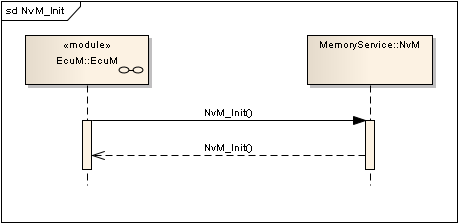
\includegraphics[scale=0.7]{Images/NvM_Init_DynamicBehavior_Overview.png}
\end{center}

NvMRead
\begin{center}
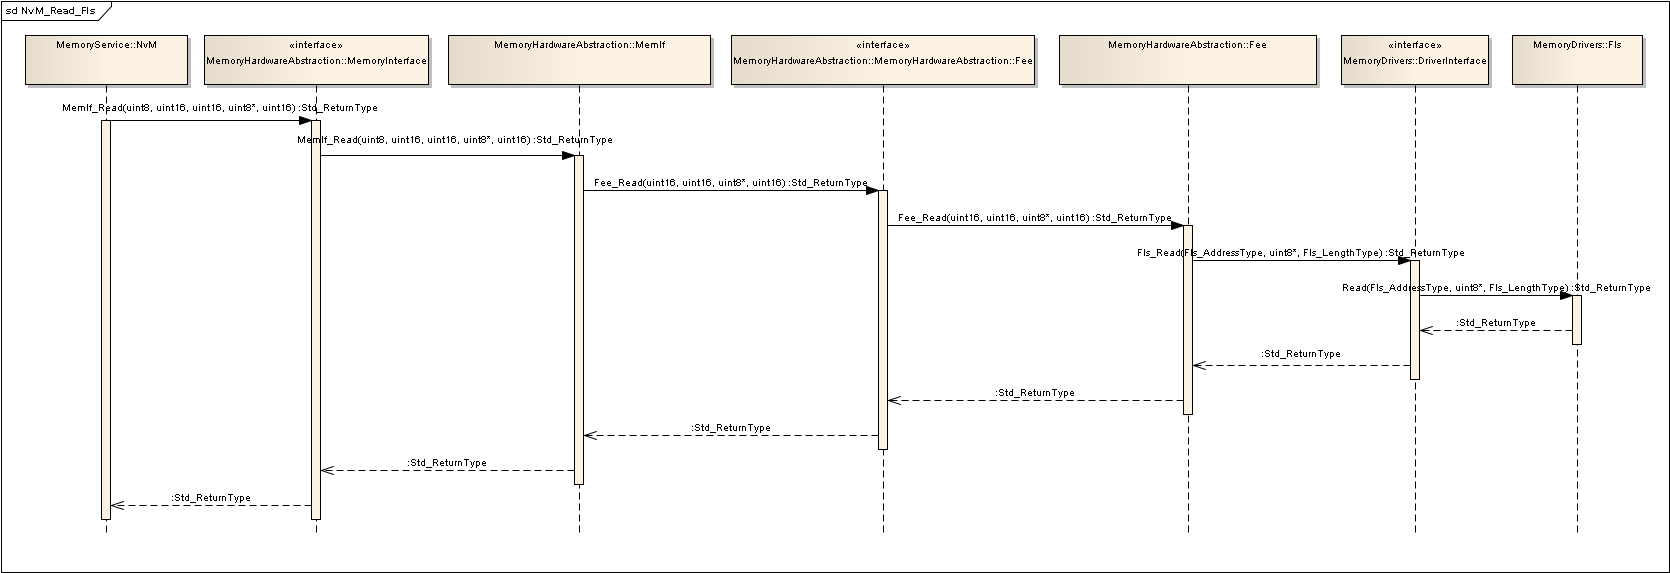
\includegraphics[scale=0.2]{Images/NvM_Read_Fls_DynamicBehavior_Overview.png}
\end{center}

NvMWrite
\begin{center}
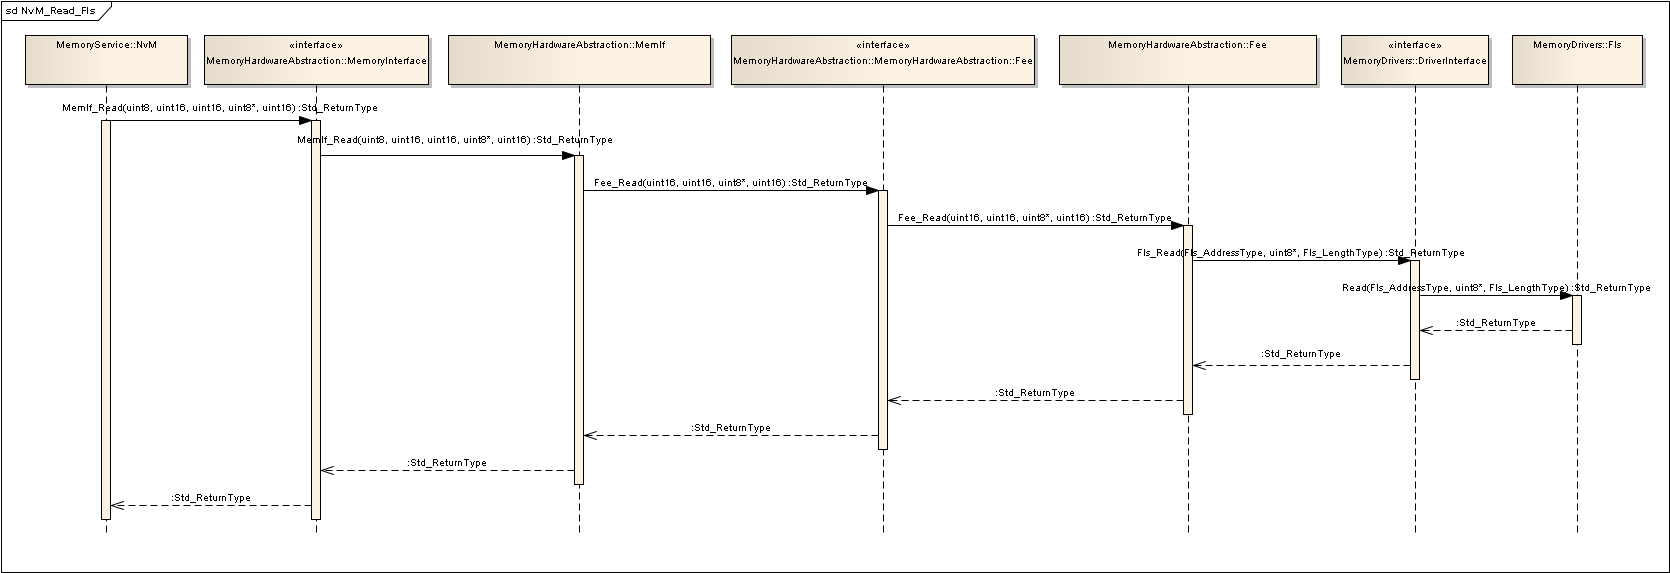
\includegraphics[scale=0.2]{Images/NvM_Read_Fls_DynamicBehavior_Overview.png}
\end{center}

\subsubsection{Reference}
